
\documentclass{article}
\usepackage[utf8]{inputenc}
\usepackage{graphicx}
\usepackage{hyperref}
\usepackage[letterpaper,margin=0.75in]{geometry}
\usepackage{setspace}

\title{Developments of a Simple Model to Elucidate the Shape of Enveloped Viruses: Motivated by Monkeypox and SARS-CoV-2}
\author{Student: Hua Deng \\ Mentor: Dr. Chwen-Yang Shew}
\date{February 21, 2025}

\begin{document}

\doublespacing
\maketitle

\begin{flushleft}
\setlength{\parindent}{45pt}

\section*{Objective}




To develop new models and simulations to study how the viral genome architecture(its shape, length and flexibility) influences the membrane. By combining polymer physics and liquid-state physics, such as crowding effects, we hope to gain a deeper understanding of viral assembly. By simulating how viral genomes behave in confined environments, we can uncover key principles behind virus formation and stability. It could contribute to more effective strategies for preventing and treating viral infections, especially for viruses like Monkeypox and SARS-CoV-2.
\section*{Introduction}

Viral infections have a critical impact on global health, emphasizing their role in pandemics and outbreaks. These infections pose significant risks to public health and encompass a wide range of diseases, from seasonal influenza to more severe infectious diseases such as Monkeypox and COVID-19. Both Monkeypox and COVID-19 viruses are classified as enveloped viruses, which are distinguished by their lipid membranes that surround and protect their genetic material (genomes). These membranes serve several crucial functions: they provide protection by shielding the viral genome from environmental factors and potential damage, and they facilitate transmission by enabling the virus to enter host cells. The membrane proteins and polysaccharides play a key role in this process by interacting with specific receptors on host cells, thereby promoting viral infection and the delivery of the genome into the host. We need to further understand these mechanisms to develop effective prevention and treatment strategies.

SARS-CoV-2, the virus responsible for COVID-19, enters a host cell by first using its spike (S) protein to bind to a specific receptor on the surface of human cells called ACE2 (angiotensin-converting enzyme 2). This spike protein acts like a key, allowing the virus to attach tightly to the host cell. After attachment, the virus enters the cell either through direct fusion with the cell membrane or via endocytosis. Once inside, the viral envelope is removed (a process called uncoating), releasing its positive-sense single-stranded RNA genome into the host cell’s cytoplasm. This viral RNA acts directly as messenger RNA (mRNA) and is translated by the host's ribosomes to produce viral proteins, including more spike proteins, structural proteins, and enzymes necessary for viral replication. The viral genome is also copied to make more RNA strands. These components are then assembled into new viral particles. Finally, the new viruses are released from the cell by budding, often taking a piece of the host’s membrane with embedded spike proteins, allowing them to infect new cells. The spike protein is essential for both the entry of the virus and for determining which cells it can infect.

Viruses often have highly symmetrical structures, such as icosahedrons (20-sided shapes). This symmetry helps distribute internal pressure evenly across the viral capsid, preventing weak spots and making the virus stable and protective of its genetic material.

When a virus infects a host, it deliberately breaks this symmetry. Doing so creates weaker areas on the surface of the capsid, which then open up to allow the virus to inject its genetic material (RNA or DNA) into the host cell. In this way, breaking symmetry is an essential part of the infection mechanism.\\


In our previous study, we developed a simple yet insightful model to understand how monomers can self-organize into trimers and tetramers on spherical surfaces. Our findings show that trimers are easier to form and more stable than dimers, and in many conditions, they are as stable—or even more stable—than tetramers. Tetramers require stronger attractive forces to form and are more prone to aggregation when these forces become too strong. These results highlight the importance of both energetic and entropic contributions to self-organization, particularly how interaction geometry and asymmetry influence the outcome.



\begin{figure}[h!]
  \centering
  \includegraphics[width=0.8\textwidth,height=4.4cm]{spike.trimer.png}
  \caption{Left image: Simulation of the SARS-CoV-2 spike protein on a spherical surface, illustrating the progression from randomly distributed monomers (left) to trimer (center) and tetramer (right) formations. Right image: SARS-CoV-2 for Covid-19 schematic image ( CDC Public
Health Image Library)}
\end{figure}

Beyond virus-related modeling, we also explored how rod-like molecules behave inside confined spaces, such as droplets or cavities, under molecular crowding. These simulations revealed that shorter rods tend to accumulate near the boundary, while longer rods align in the interior—behaviors that closely match experimental observations. Altogether, our work provides a foundation for understanding how structure and organization emerge in complex systems.


\begin{figure}[!ht]
  \centering
   \includegraphics[width=0.8\textwidth,height=5.5cm]{F-actin.png}
 
  \caption{\textbf{Left image:} Short DNA rods distribute near wall under molecular crowding. Long F-actin rods distribute in cavity interior and show high orientation ordering. Long F-actin rods distribute in cavity interior and show high orientation ordering.  Specific localization of 
  long DNA ($\lambda$ DNA) and F-actin in DEX-rich CAMDs.    
       \textbf{Right image:} Fluorescence microscopic images of DNA (GelGreen), actin (Alexa Fluor 546), and merged views are shown, along with polarization microscopy observations (four panels on the left). 
        The images were captured under the conditions of 120~$\mu$M $\lambda$ DNA, 10~$\mu$M actin, and 4.0~mM KCl. 
        F-actins were observed to be in a nematic liquid-crystal state at the center of DEX-rich CAMDs, while DNA molecules appeared segregated from the center. 
        In other words, long DNA strands are compressed by the aligned F-actin region, as schematically illustrated in the right panel. 
        Scale bar: 100~$\mu$m.}
\end{figure}

\section*{Background} 
The genomic material of SARS-CoV-2 (single-stranded RNA) and Monkeypox (double-stranded DNA) behaves like a polymer. 


\subsection*{I. Polymer}
The polymer is a large molecule composed of identical monomers or different types of monomers linked by covalent bonds. Both RNA and DNA are composed of long sequences of nucleotides linked together by phosphodiester bonds. 

\begin{figure}[!ht]
  \centering
  
  \fbox{\includegraphics[width=0.4\textwidth,height=2.5cm]{polymer.png}}
  \caption{Polymer}
\end{figure}





\subsection*{II. Membrane/Phospholipids}
Phospholipids are the main ingredients of cell and viral membranes, and their structure is actually a lot like a simple polymer. Each one has a head that loves water and two tails that hate it. The head is connected to the tails through a small backbone, so the whole molecule looks kind of like a


\begin{figure}[!ht]
  \centering
  \fbox{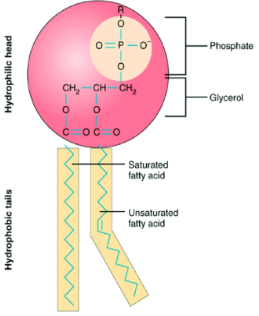
\includegraphics[width=0.35\textwidth,height=7cm]{membrane.png}}
  \caption{membrane subunit}
\end{figure}






\noindent matchstick or a two-tailed kite. Because one part of the molecule wants to be near water and the other part wants to avoid it, phospholipids naturally arrange themselves into layers when they’re in water. These layers form flexible membranes that act a lot like soft polymer sheets—they can bend, move, and even stretch a little. In fact, scientists often use ideas from polymer physics to study how these membranes behave, especially when trying to understand things like how viruses wrap themselves up or how they enter cells.




\subsection*{III. Genome/DNA/RNA}
DNA and RNA are long chains made up of smaller units called nucleotides. Each nucleotide is like a puzzle piece, made of a sugar, a phosphate group, and a nitrogen base. In DNA, the sugar is called deoxyribose, and in RNA, it’s ribose. The bases are the parts that carry genetic 

\begin{figure}[!ht]
  \centering
  
   \fbox{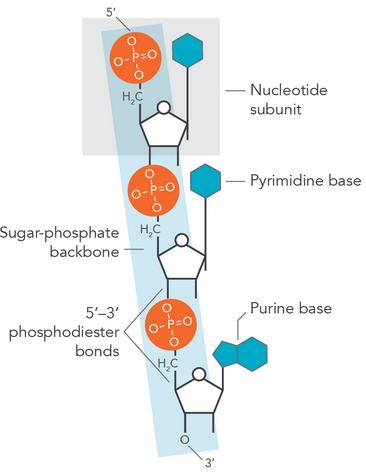
\includegraphics[width=0.35\textwidth,height=8cm]{genome.png}}

  \caption{Nucletide subunits}
\end{figure}


\noindent information—A, T, G, and C in DNA, and A, U, G, and C in RNA (with U replacing T in RNA). These nucleotides link together through bonds between the phosphate of one and the sugar of the next, forming a backbone, kind of like beads on a string. 





Nucleotides, the building blocks of RNA and DNA, act as repeating units  that form larger macromolecules, similar to how polymers are made from repeating monomers. The polymeric nature allows genomic material to adopt different shapes and configurations. Just as polymers can interact with other compounds, RNA and DNA can form secondary structures and interact with proteins, which is essential for processes like gene expression and viral assembly. Polymers can have various structures—linear, branched, or crosslinked—allowing them to be flexible, adaptable, and capable of forming diverse shapes and configurations.  DNA and RNA are biopolymers, and it means they have a polymeric nature that enables them to fold, coil, and interact with other molecules based on factors like sequence, chemical interactions, and environmental conditions.



This makes DNA and RNA behave like polymers—long, repeating chains that can twist, bend, and fold. DNA usually forms a double helix, with two strands held together by base pairing (A with T, and G with C), while RNA is usually single-stranded and folds into all kinds of shapes. In science, especially in physics, we can think of DNA and RNA as flexible polymers, which helps us understand how they fold up inside tiny spaces—like the inside of a virus.



\subsection*{IV. Protein/Amino Acid chain}
Proteins are natural polymers made up of amino acids, which are like the individual links in a chain. Each amino acid has the same basic structure: a central carbon atom (called the alpha carbon) bonded to a hydrogen, an amino group (–NH$_2$), a carboxyl group (–COOH), and a unique side chain, known as the R group. These amino acids connect through peptide bonds, forming a 

\begin{figure}[h!]
  \centering
   \fbox{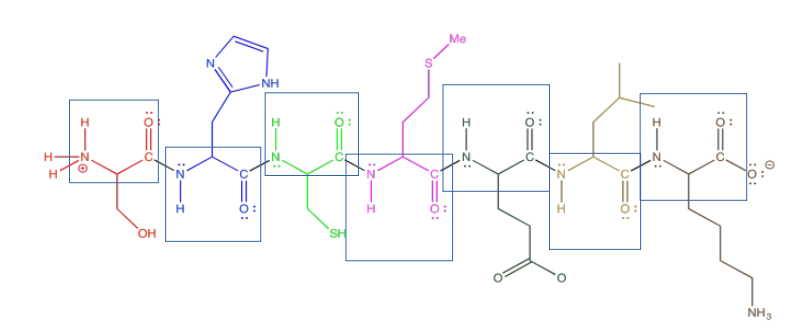
\includegraphics[width=0.5\textwidth,height=4cm]{protein.png}}
  
  %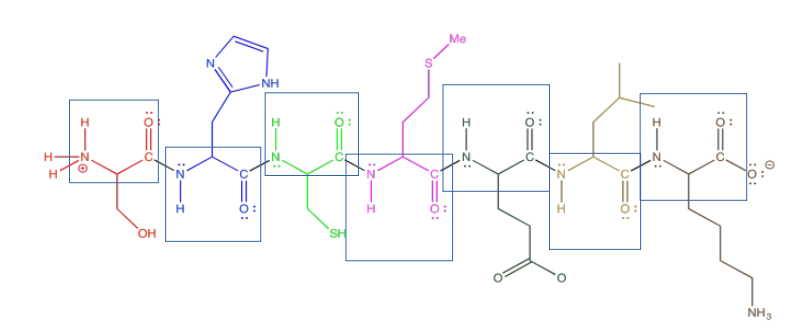
\includegraphics[width=0.5\textwidth,height=4cm]{protein.png}  % Adjust width or height as needed
  \caption{Amino acid chain}
\end{figure}

\noindent backbone that repeats along the entire length of the chain—just like a synthetic polymer has repeating units. But proteins don’t stay as simple straight chains. They start folding right away into more complex shapes. First, they form local patterns like alpha helices (coils) and beta sheets (pleated folds), which are stabilized by hydrogen bonds. Then the entire chain folds into a specific 3D structure, known as the tertiary structure, shaped by interactions between the R groups—like hydrogen bonding, hydrophobic packing, or ionic attractions. Sometimes multiple folded chains come together to form a quaternary structure. This whole folding process is what makes a protein functional. So while a protein is a polymer at its core, its complexity and flexibility come from the variety in its amino acids and the way they interact in space. 



After a protein folds into its final shape, it still technically is a polymer—it’s just a much more complex and organized one. Instead of looking like a simple chain or string, a folded protein looks more like a tangled but purposeful knot or a compact 3D sculpture. The backbone of the chain is still there, repeating like in any polymer, but now it's been twisted, looped, and packed in a specific way to create a functional structure. Some parts form spirals (alpha helices), others form sheets (beta sheets), and the rest bends and loops to connect them all together. Even though it’s not as uniform-looking as a plastic polymer, it still behaves like a polymer chain in the sense that it’s made from repeating units (amino acids), it has flexibility, and it responds to its environment. So a folded protein is like a smart, dynamic polymer—one that’s shaped by chemistry, and whose final form is directly tied to its job inside the body.



The genome of the Monkeypox virus is a double-stranded DNA, approximately 190 kb (kilobases) in length, which equals about 95 kbp (kilobase pairs). This genomic length corresponds to a substantial contour length of approximately 3000 nm. This indicates that the genetic material is significantly longer than the physical dimensions of the virus itself, which measures around 250 nm long. 
These viral particles can display spherical and oval shapes, indicating different developmental stages: immature virions tend to be spherical, while mature virions adopt an oval shape. This morphological differentiation can be important for recognizing stages in the virus life cycle and understanding how these changes may affect infectivity. The transition from spherical to oval shapes may be linked to the maturation process, influencing the virus's ability to enter host cells and replicate effectively.\\

The shape of viral particles, like those seen in the Monkeypox virus, can reveal a lot about what stage they’re at in their life cycle. In the early phases, the virus forms immature virions that are usually spherical. This round shape isn’t random—it helps the virus begin assembling its genetic material and proteins in a flexible, efficient way. At this point, the virus is just starting to come together, packaging its core components. As it matures, the virus goes through structural 

\begin{figure}[h!]
  \centering
  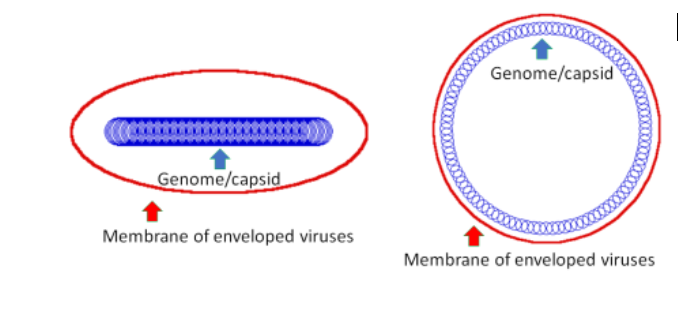
\includegraphics[width=0.5\textwidth,height=4cm]{monkeypox.png}  % Adjust width or height as needed
  \caption{Preliminary 2D model studies to
investigate the effect of the geometry of a
genome on the shape of a virus. A rod-like
genome induces an elliptic shape whereas a
circular genome leads to a circular shape.}
\end{figure}

\noindent changes that shift its shape from spherical to oval. This transformation involves the rearrangement of viral proteins, which makes the particle more stable. The oval shape not only helps the mature virion survive better outside the host but also improves its ability to attach to and enter host cells. This increased stability and better interaction with host cell receptors make the mature, oval-shaped virus more infectious and better equipped to replicate once inside a host.

\section*{Method} 
\subsection*{1 Models}
\subsection*{1.1 Coase-grain model}

\subsection*{1.1.1 Adveantage of Coase-grain model}
	Using a coarse-grain model in polymer science is really helpful because it makes things simpler and more efficient, especially when dealing with large and complex systems. One of the biggest reasons to use coarse-graining is that it saves a lot of computational power. Polymers are often made up of thousands or even millions of atoms, so simulating each individual atom takes a huge amount of time and resources. Instead of modeling each atom, a coarse-grain model groups several atoms or monomers into a "bead," which reduces the number of particles in the simulation. This allows researchers to study bigger systems and longer timescales without overwhelming their computers.

	Another advantage is that coarse-graining allows scientists to focus on the big picture of polymer behavior. At the atomic level, polymers have tons of detailed interactions, but often what we care about are the overall properties, like how the polymer stretches, bends, or reacts to forces. Coarse-graining simplifies this by letting researchers study these larger-scale behaviors without getting caught up in the tiny atomic details, which are often less important for understanding real-world polymer behavior.
	
	Coarse-grain models also make it easier to model interactions between polymers. Instead of focusing on each individual monomer, coarse-graining represents groups of monomers as beads. This makes the interactions between polymer chains less complex and easier to study. This is really useful for studying complicated systems like polymer networks, gels, or blends, which would be too difficult to model atom by atom.\\
	
	
	Another reason coarse-grain models are so valuable is that they help researchers simulate larger systems over longer periods of time. By reducing the number of particles in the model, simulations can run much faster and allow for studies over longer timescales. Instead of simulating each tiny atom’s movement, which can take a long time, coarse-graining lets researchers study the overall behavior of the polymer chain over much longer periods. This is really useful for looking at things like polymerization processes or phase transitions that occur over time.
	
	Coarse-grain models also focuses on the important polymer properties that matter most, like flexibility, shape changes, and how polymers self-assemble. These properties are often determined by the overall structure of the polymer, not by the exact positions of every single atom. So by simplifying the model, researchers can study how polymers fold, how they form membranes, or how they interact with other molecules, without having to get into the nitty-gritty of atomic-level details.\\
	
	Finally, coarse-grain models are essential for designing new materials. When scientists are developing new types of polymers—whether for drug delivery, biodegradable plastics, or high-performance materials—these models help predict how the polymer will behave in different environments. This helps researchers optimize the materials for real-world uses without needing to simulate every tiny detail.
	In the end, coarse-grain models are incredibly useful in polymer science because they simplify complex systems, making it easier to study their behavior. They save time and computational power while still allowing scientists to focus on the big picture—like how polymers stretch, bend, and interact—helping to design better materials and understand how polymers work in the real world.


\subsection*{1.1.2 Assumption of Coarse grain model}
Coarse-grained models come with several assumptions that are critical for their application:\\
    1. Homogeneity:\\
    It is often assumed that the system is uniform, meaning properties do not vary significantly across space. \\
    2. Bead Representation:\\
        Each bead represents a group of atoms, assuming they behave as a single entity in terms of interactions, which may not always reflect the nuances of molecular behavior. \\
    3. Simplified Interactions:\\
        The models typically ignore specific interactions at the atomic level, such as hydrogen bonding or van der Waals forces, unless they are effective at the coarse-grained level. \\
    4. Mean-Field Approximations:\\
        Coarse-grained models often use mean-field approximations, averaging the effects of all other particles on any given particle, simplifying the interactions that can be complex in real systems. \\
    5. Fixed Connectivity:\\
        In polymer applications, it usually assumes fixed connectivity between beads, which may not fully account for the flexibility in the actual polymer chains. \\ 

\subsection*{1.2 Simple liquid Models}

Simple liquid models that help understand the structure and behavior of polymer fluids in crowded environments. Specifically, the simple liquid models referenced include Hard Sphere Model and Lennard-Jones Model. 


Hard sphere model is used to understand the behavior of particles in crowded environments, where the excluded volume effect becomes important. 


The Lennard-Jones model accounts for both attractive and repulsive forces between particles, which is important in understanding the interactions within fluids and condensed matter. It helps model the behavior of molecules, especially in non-ideal conditions like those found in crowded environments. 
\subsection*{1.3 Summary of the models}
Coarse-grain model and simple liquid models are valuable tools in understanding how particles interact in condensed matter systems, such as polymer fluids, from both an energetic (energy of interactions) and entropic (disorder and randomness) perspective.


\subsection*{II.Simulation}


\subsection*{1.1 Monto Carlo simulation}

Monte Carlo (MC) simulation is a technique used to explore different configurations of a system by randomly sampling possible states, based on probability rules that often relate to energy. Instead of following every tiny movement of particles over time—like molecular dynamics does—Monte Carlo takes a different approach. It “jumps” from one possible state to another and decides whether to accept or reject each move depending on how favorable it is, typically using criteria like energy minimization.
This method becomes especially powerful when combined with coarse-grain (CG) models. Coarse-graining simplifies complex systems by grouping atoms or monomers into larger units, reducing the number of particles and interactions. This makes the system easier and faster to simulate, which is perfect for Monte Carlo techniques. With fewer variables to track, MC simulations can explore a much wider range of configurations in less time.
Using MC with CG models is particularly useful for studying large-scale behaviors like polymer folding, self-assembly, phase transitions, or how polymers interact with other surfaces or structures. Since you don’t need to worry about every atomic detail, you can focus on understanding the broader behavior of the material. For instance, in a coarse-grain polymer simulation, MC methods might rotate parts of the polymer chain, stretch or shift segments, or rearrange them—checking each time how these changes affect the system’s overall energy or structure.
In short, Monte Carlo simulations and coarse-grain modeling work hand in hand. Together, they make it possible to study complex polymer systems more efficiently and gain insights that would be hard to reach using more detailed, atomistic approaches.

\subsection*{1.2 Assumpations of Monto Carlo simulation}


    1. Randomness is representative
    
The simulation assumes that the random inputs it uses (often generated using pseudo-random number generators) adequately represent the variability and uncertainty of real-life scenarios.\\

\noindent 2. Independent trials
    
Each simulation run (or trial) is assumed to be independent of the others. The outcome of one run does not affect the outcome of another.

\noindent    3. Known probability distributions
    
The input variables must follow known probability distributions (e.g., normal, uniform, triangular, etc.). The accuracy of the results relies heavily on how well these distributions reflect real-world behavior.

\noindent  4. Large number of iterations
    
The law of large numbers is a key assumption — with a large enough number of trials, the average of the simulated outcomes should approximate the expected value. More iterations generally improve accuracy.

\noindent5. System/process remains stable
    
The simulation assumes that the underlying process or system doesn’t change over time during the simulation (i.e., it's stationary).

\noindent    6. Model structure is correct

The simulation is only as good as the model it's based on. It assumes the mathematical or logical structure you build reflects the real-world process correctly.

\subsection*{III. Summary}
Viral genomes (like those in Monkeypox and SARS-CoV-2) behave similarly to a polymer chain packed inside a small, crowded space (the viral capsid/membrane). The project aims to extend existing models and Monto Carlo simulation to study how the genome's architecture (shape, length, and flexibility) affects the overall shape of a virus. This will help us understand how viral genomes and membranes interact, which is crucial for predicting viral structures and behavior.






\begin{equation}
E = -\Gamma \frac{\exp(-\kappa_1 r)}{r} + \int \left( \frac{\kappa_2}{2} (C_1 + C_2 - C_0)^2 + \sigma \right) dA 
\end{equation}

\(\Gamma\) is the interaction strength,\\
\(\kappa_1\) is the screening parameter \\
\(\kappa_2\) is bending rigidity (determines how resistant the membrane is to bending) \\
\(r\) is the distance, \\
\(C_1\), \(C_2\) are the principal curvatures, of the membraneat each point\\
\(C_0\) is the spontaneous curvature, which represents the preferred cuvaturea due to asymmetry in the membrane
\(\sigma\) is the surface tension(accounts for the energy cost of increasing the membrane area)\\
\(dA\) is the differential area element(integrates energy over the entire membrane surface)\\




\end{flushleft}



\end{document}




